% !TEX program = xelatex
% ---------------------------------------------------------------------------
%  The Origin of Origins  —  a short note
%  Compile with:  xelatex origin_of_origins.tex   (twice)
%  Figures: fig1_origins.pdf, fig2_unique.pdf, fig3_squares.pdf (figs_origins.py), fig4_spirals.png
%  Exact checks: verify_origins.py
% ---------------------------------------------------------------------------
\documentclass[11pt,a4paper]{article}

\usepackage[margin=2.6cm]{geometry}
\renewcommand{\topfraction}{0.9}\renewcommand{\bottomfraction}{0.8}\renewcommand{\textfraction}{0.07}\renewcommand{\floatpagefraction}{0.8}
\usepackage{amsmath,amsthm,mathtools}
\usepackage{fontspec}
\usepackage{unicode-math}
\setmainfont{Latin Modern Roman}
\setmathfont{Latin Modern Math}
\newfontfamily\greekfont{GFS Porson}[Scale=MatchLowercase]
\usepackage{graphicx}
\usepackage{enumitem}
\usepackage{xcolor}
\usepackage[hidelinks]{hyperref}
\usepackage{caption}
\captionsetup{font=small,labelfont=bf}

\newcommand{\gr}[1]{{\greekfont #1}}

\theoremstyle{plain}
\newtheorem{theorem}{Theorem}
\newtheorem{proposition}[theorem]{Proposition}
\newtheorem{corollary}[theorem]{Corollary}
\theoremstyle{definition}
\newtheorem{definition}[theorem]{Definition}
\theoremstyle{remark}
\newtheorem{remark}[theorem]{Remark}

\hypersetup{
  pdftitle={The Origin of Origins},
  pdfauthor={Lluis Garcia Torcal},
  pdfkeywords={Fibonacci tiling, Holden's lines, golden spiral, circle of origins, 3-4-5 triangle, dihedral symmetry}
}

\begin{document}

\begin{center}
{\LARGE The Origin of Origins\par}
\vspace{0.3em}
{\large How a circle of area $\pi/10$ about the centre of the unit square gives eight origins,\\[2pt] one for each of eight Fibonacci spirals: four, and their four mirror images\par}
\vspace{1.2em}
{\large Lluis Garcia Torcal\par}
\vspace{0.3em}
{\small Independent researcher, Sabadell, Spain \quad·\quad ORCID \href{https://orcid.org/0009-0007-8570-2536}{0009-0007-8570-2536}\\ \href{mailto:lluisgarciamusic@gmail.com}{lluisgarciamusic@gmail.com}\par}
\vspace{0.3em}
{\small Version 1, October 2026\par}
\end{center}

\vspace{0.8em}
\begin{abstract}
\noindent We start from one point, the centre $O$ of the unit square, the \emph{origin of origins}. Each \emph{diagonal arc} of the square, the quarter of the circle of radius $1$ about one corner that joins the two opposite corners next to it, meets a circle about $O$ whenever the radius lies between $1-\sqrt{2}/2$ and $\sqrt2/2$. We prove that exactly one of these circles has the following property: the tangent at a crossing with a diagonal arc passes through an end of that arc, a corner of the square other than the crossing itself. It is the circle of radius $\sqrt{0.1}$, which we call the \emph{origins unit}, and of area exactly $\pi/10$: one tenth of the circle of radius $1$ that the diagonal arcs come from. We call it the \emph{circle of origins}. It meets the four diagonal arcs in eight points, $(\pm\tfrac{3}{10},\pm\tfrac1{10})$ and $(\pm\tfrac1{10},\pm\tfrac3{10})$, the \emph{eight origins}. The eight symmetries of the square turn the Fibonacci tiling into eight tilings, each with its own spiral (four, and their four mirror images), and each of the eight origins belongs to one of them. In connection with the two lines through the centres of the squares found by Holden (1975): the crossing of the lines is an origin, lying on a diagonal arc; one line is the tangent of the circle of origins there, which passes through an end of that arc, and the other is the perpendicular there, which runs through $O$ to the opposite origin. Seen from $O$, consecutive origins are $\arctan(4/3)$ and $\arctan(3/4)$ apart, the angles of the $3$-$4$-$5$ triangle, and enclose areas of exactly $3/100$ and $4/100$; alternate origins form two squares of area $1/5$, whose eight crossing points are the vertices of two squares, of areas $1/8$ and $1/9$. All statements are elementary; the rational ones are verified in exact arithmetic.
\end{abstract}

\section{Setting and names}

The unit square has its centre at $O=(0,0)$ and corners $(\pm\tfrac12,\pm\tfrac12)$; we write $E=(\tfrac12,\tfrac12)$. For a corner $K$, the \emph{diagonal arc} $A_K$ is the quarter of the circle of radius $1$ about $K$ that joins the two corners next to $K$. These two corners are opposite corners of the square, so $A_K$ is a curved diagonal; its ends $E'$ satisfy $E'\cdot K=0$ and $|E'|^2=\tfrac12$. The four diagonal arcs are drawn in Figure~\ref{fig:origins}. The Fibonacci spiral is made of such arcs, one in each square of the tiling; in the first square it is one of these four.

We build the tiling by attaching squares of sides $1,1,2,3,5,8,\dots$ below, to the right, above and to the left, in turn; the centres are $C_1=(0,0)$, $C_2=(0,-1)$, $C_3=(\tfrac32,-\tfrac12)$, $C_4=(1,2)$, $C_5=(-3,1)$, \dots. Holden \cite{holden} proved that the centres lie alternately on two perpendicular lines, of slopes $3$ and $-1/3$ whatever the first two sides, and gave their distances from the crossing of the lines in closed form, $d_i=(f_{i+3}+f_{i-3})/(2\sqrt{10})$, with $d_{i+2}=d_{i+1}+d_i$; his tables list $d\sqrt{10}$, which for the Fibonacci tiling are $3,4,7,11,18,\dots$. Gardiner \cite{gardiner} gave the lines in coordinates centred on the first square, as $y=3x$ and $3y=-(x-1)$, whose crossing is at $(\tfrac1{10},\tfrac3{10})$, at distance $1/\sqrt{10}$ from that centre. Our frame is Gardiner's turned a quarter turn about $O$, and in it the lines are
\[
  x+3y=0 \qquad\text{and}\qquad 3x-y=1,
\]
which cross at $H_0=(\tfrac3{10},-\tfrac1{10})$, and $|C_kH_0| = L_k/\sqrt{10}$, where $L_k=1,3,4,7,11,\dots$ are the Lucas numbers: with Fibonacci sides, Holden's closed form and the identity $F_{n+3}+F_{n-3}=2L_n$ give exactly $L_k/\sqrt{10}$, (Holden's $f_i$ is our $F_{i+1}$, so his index $i$ is our $k-1$), though Holden does not name the Lucas numbers; for the first square, directly, $|C_1H_0|=|H_0|=1/\sqrt{10}$. We keep the name \emph{Holden's lines} for these two lines and \emph{Holden's crossing} for $H_0$, which is what Holden found. Following Gardiner \cite{gardiner}, who numbered the squares from the first, we call $x+3y=0$, through the centres of the odd-numbered squares, the \emph{odd line}, and $3x-y=1$, through the centres of the even-numbered squares, the \emph{even line}.

\paragraph{Names.} We call $O$ the \emph{origin of origins} (\gr{ἡ ἀρχὴ τῶν ἀρχῶν}). The circle about $O$ of radius $\rho=\sqrt{0.1}=1/\sqrt{10}$ we call the \emph{circle of origins} (\gr{ὁ κύκλος τῶν ἀρχῶν}); its area is $\pi\rho^2=\pi/10$, exactly one tenth of the area $\pi$ of the circle of radius $1$ that the diagonal arcs come from, and its circumference is $2\pi/\sqrt{10}$. The eight points where it meets the diagonal arcs (Corollary~\ref{cor:origins}) we call the \emph{eight origins}, because they are the points from which lengths are counted in steps of $\rho$: each origin is exactly one step from $O$, and in each of the eight tilings the centres of the squares are a whole number of steps, $L_k$, from its origin (as above, and Section~3). We therefore call $\rho$ the \emph{origins unit}. In \cite{rhombus} the same length was called the Holden unit; the reason for the new name is given in Remark~\ref{rem:credit}.

\section{The circle of origins}

A circle about $O$ of radius $r$ meets the diagonal arc $A_K$ exactly when $1-\tfrac{\sqrt2}{2}\le r\le \tfrac{\sqrt2}{2}$: the arc comes closest to $O$ at its midpoint, at distance $1-|K| = 1-\tfrac{\sqrt2}2\approx 0.293$, and is farthest at its ends, at distance $\tfrac{\sqrt2}2$. For every such radius there is a crossing, and a tangent to the circle there. Only one radius makes that tangent go through an end of the arc.

\begin{figure}[t]
\centering
\begin{minipage}[t]{0.48\textwidth}\centering
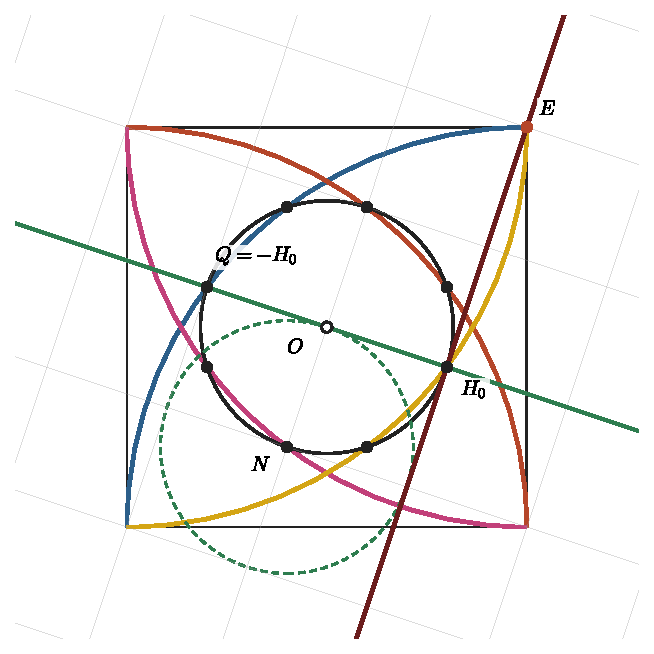
\includegraphics[width=0.86\textwidth]{fig1_origins.pdf}
\caption{The four diagonal arcs, the circle of origins and the eight origins. At $H_0$ the tangent of the circle, the even line (dark red), passes through the corner $E$. The odd line (green) is the perpendicular at $H_0$, through $O$ to the opposite origin $Q$, and also the tangent at $O$ of the equal circle about the origin $N$ (dashed). These are Holden's lines; the origins grid, of side $\rho$, is shown faintly.}
\label{fig:origins}
\end{minipage}\hfill
\begin{minipage}[t]{0.48\textwidth}\centering
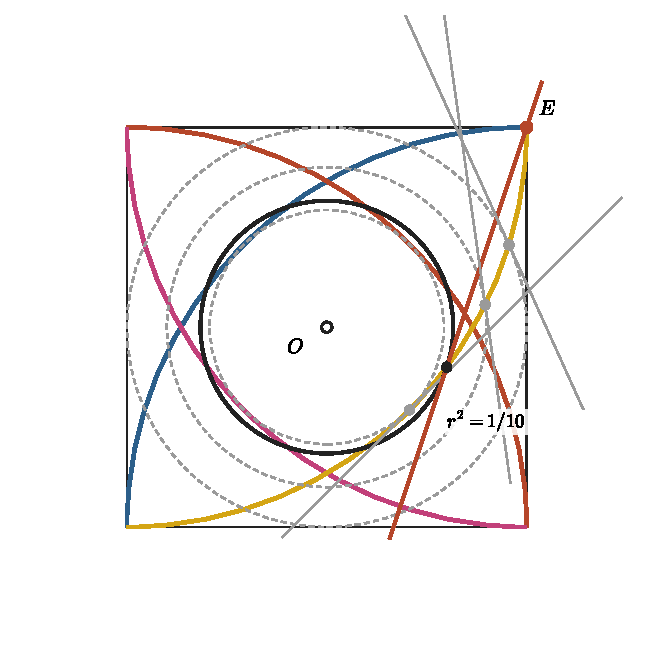
\includegraphics[width=0.86\textwidth]{fig2_unique.pdf}
\caption{Circles about $O$ of other radii (dashed), with the tangent at their crossing with the same diagonal arc (grey). Only for $r^2=1/10$ does the tangent pass through the corner $E$. The smallest circle just touches the arc ($r=1-\sqrt2/2$).}
\label{fig:unique}
\end{minipage}
\end{figure}

\begin{theorem}\label{thm:unique}
Let $p$ be a point where the circle $|p|=r$ meets the diagonal arc $A_K$. The tangent to the circle at $p$ passes through an end of $A_K$ if and only if
\[
  20r^4-12r^2+1=0, \qquad\text{that is}\qquad r^2=\tfrac1{10}\ \text{ or }\ r^2=\tfrac12 .
\]
For $r^2=\tfrac12$ the crossing $p$ is that end itself, so the condition holds only trivially. The circle of origins is therefore the only circle about $O$ whose tangent at a crossing with a diagonal arc passes through an end of that arc other than the crossing itself.
\end{theorem}

\begin{proof}
Write $t=r^2$. From $|p-K|^2=1$, $|p|^2=t$ and $|K|^2=\tfrac12$ we get $p\cdot K=\tfrac12(t-\tfrac12)$. The tangent at $p$ is the line $x\cdot p=t$; it passes through the end $E'$ exactly when $p\cdot E'=t$. Since $K$ and $E'$ are perpendicular and both of length $1/\sqrt2$, $p=2(p\cdot K)\,K+2(p\cdot E')\,E'$, so
\[
  t=|p|^2 = 2(p\cdot K)^2 + 2(p\cdot E')^2 = \tfrac12\bigl(t-\tfrac12\bigr)^2 + 2t^2 ,
\]
which is $20t^2-12t+1=0$, with roots $t=\tfrac1{10}$ and $t=\tfrac12$ (discriminant $64=8^2$). For $t=\tfrac12$, $p\cdot K=0$ and $p\cdot E'=\tfrac12$, so $p=E'$. Conversely, for each root the point $p=2(p\cdot K)K+2tE'$ lies on both circles, and on the quarter arc $A_K$ itself: for $t=\tfrac1{10}$ and $K=(-\tfrac12,\tfrac12)$, $E'=E$, it is $p=(\tfrac3{10},-\tfrac1{10})$, with $p-K=(\tfrac45,-\tfrac35)$ between the directions $(1,0)$ and $(0,-1)$ of the two ends; the other cases follow by the symmetries of the square.
\end{proof}

\begin{remark}
The trivial root $r^2=\tfrac12$ is the circle through the four corners. It meets the diagonal arcs only at their ends, so it gives four points, not eight, and its tangents there have slopes $\pm1$ (for example $y=x+1$ at the corner $(-\tfrac12,\tfrac12)$): they are not lines of the origins grid, and none of them is one of the two lines of Holden's theorem for any of the eight tilings (those have slopes $\pm3$ and $\pm\tfrac13$: $3$ and $-\tfrac13$ for the four rotations, $-3$ and $\tfrac13$ for the four reflections). Its radius $\sqrt{1/2}=\sqrt5\,\rho$ is the diagonal of two cells of the origins grid side by side, since $(-\tfrac12,\tfrac12) = -2\,(\tfrac3{10},-\tfrac1{10}) + (\tfrac1{10},\tfrac3{10})$.
\end{remark}

\begin{remark}
The other two corners are not ends of $A_K$. The tangent can never pass through $K$ itself ($p\cdot K=t$ would need $t=-\tfrac12$). It does pass through the far corner $-K$ when $p\cdot(-K)=t$, that is $t=\tfrac16$; but then $p\cdot E'=\pm 1/(3\sqrt2)$, so this crossing has irrational coordinates and is not a node of the origins grid (Section~3). Figure~\ref{fig:unique} shows circles of other radii: their tangents miss the end $E$ of the arc.
\end{remark}

\begin{corollary}[the eight origins]\label{cor:origins}
For $r^2=\tfrac1{10}$ the crossings are $p=-\tfrac25K+\tfrac15E'$, two on each diagonal arc (one for each end):
\[
  \bigl(\pm\tfrac3{10},\pm\tfrac1{10}\bigr)\quad\text{and}\quad\bigl(\pm\tfrac1{10},\pm\tfrac3{10}\bigr),
\]
eight points in all. We call them the \emph{eight origins}. The circle of origins meets the diagonal arcs nowhere else, and its area is $\pi\rho^2=\pi/10$.
\end{corollary}

\begin{proof}
Put $t=\tfrac1{10}$ in $p=2(p\cdot K)K+2(p\cdot E')E'$, with $p\cdot K=-\tfrac15$ and $p\cdot E'=\tfrac1{10}$. The circles $|p|^2=\tfrac1{10}$ and $|p-K|^2=1$ meet only on the line $p\cdot K=-\tfrac15$, so in at most two points.
\end{proof}



\begin{figure}[!b]
\centering
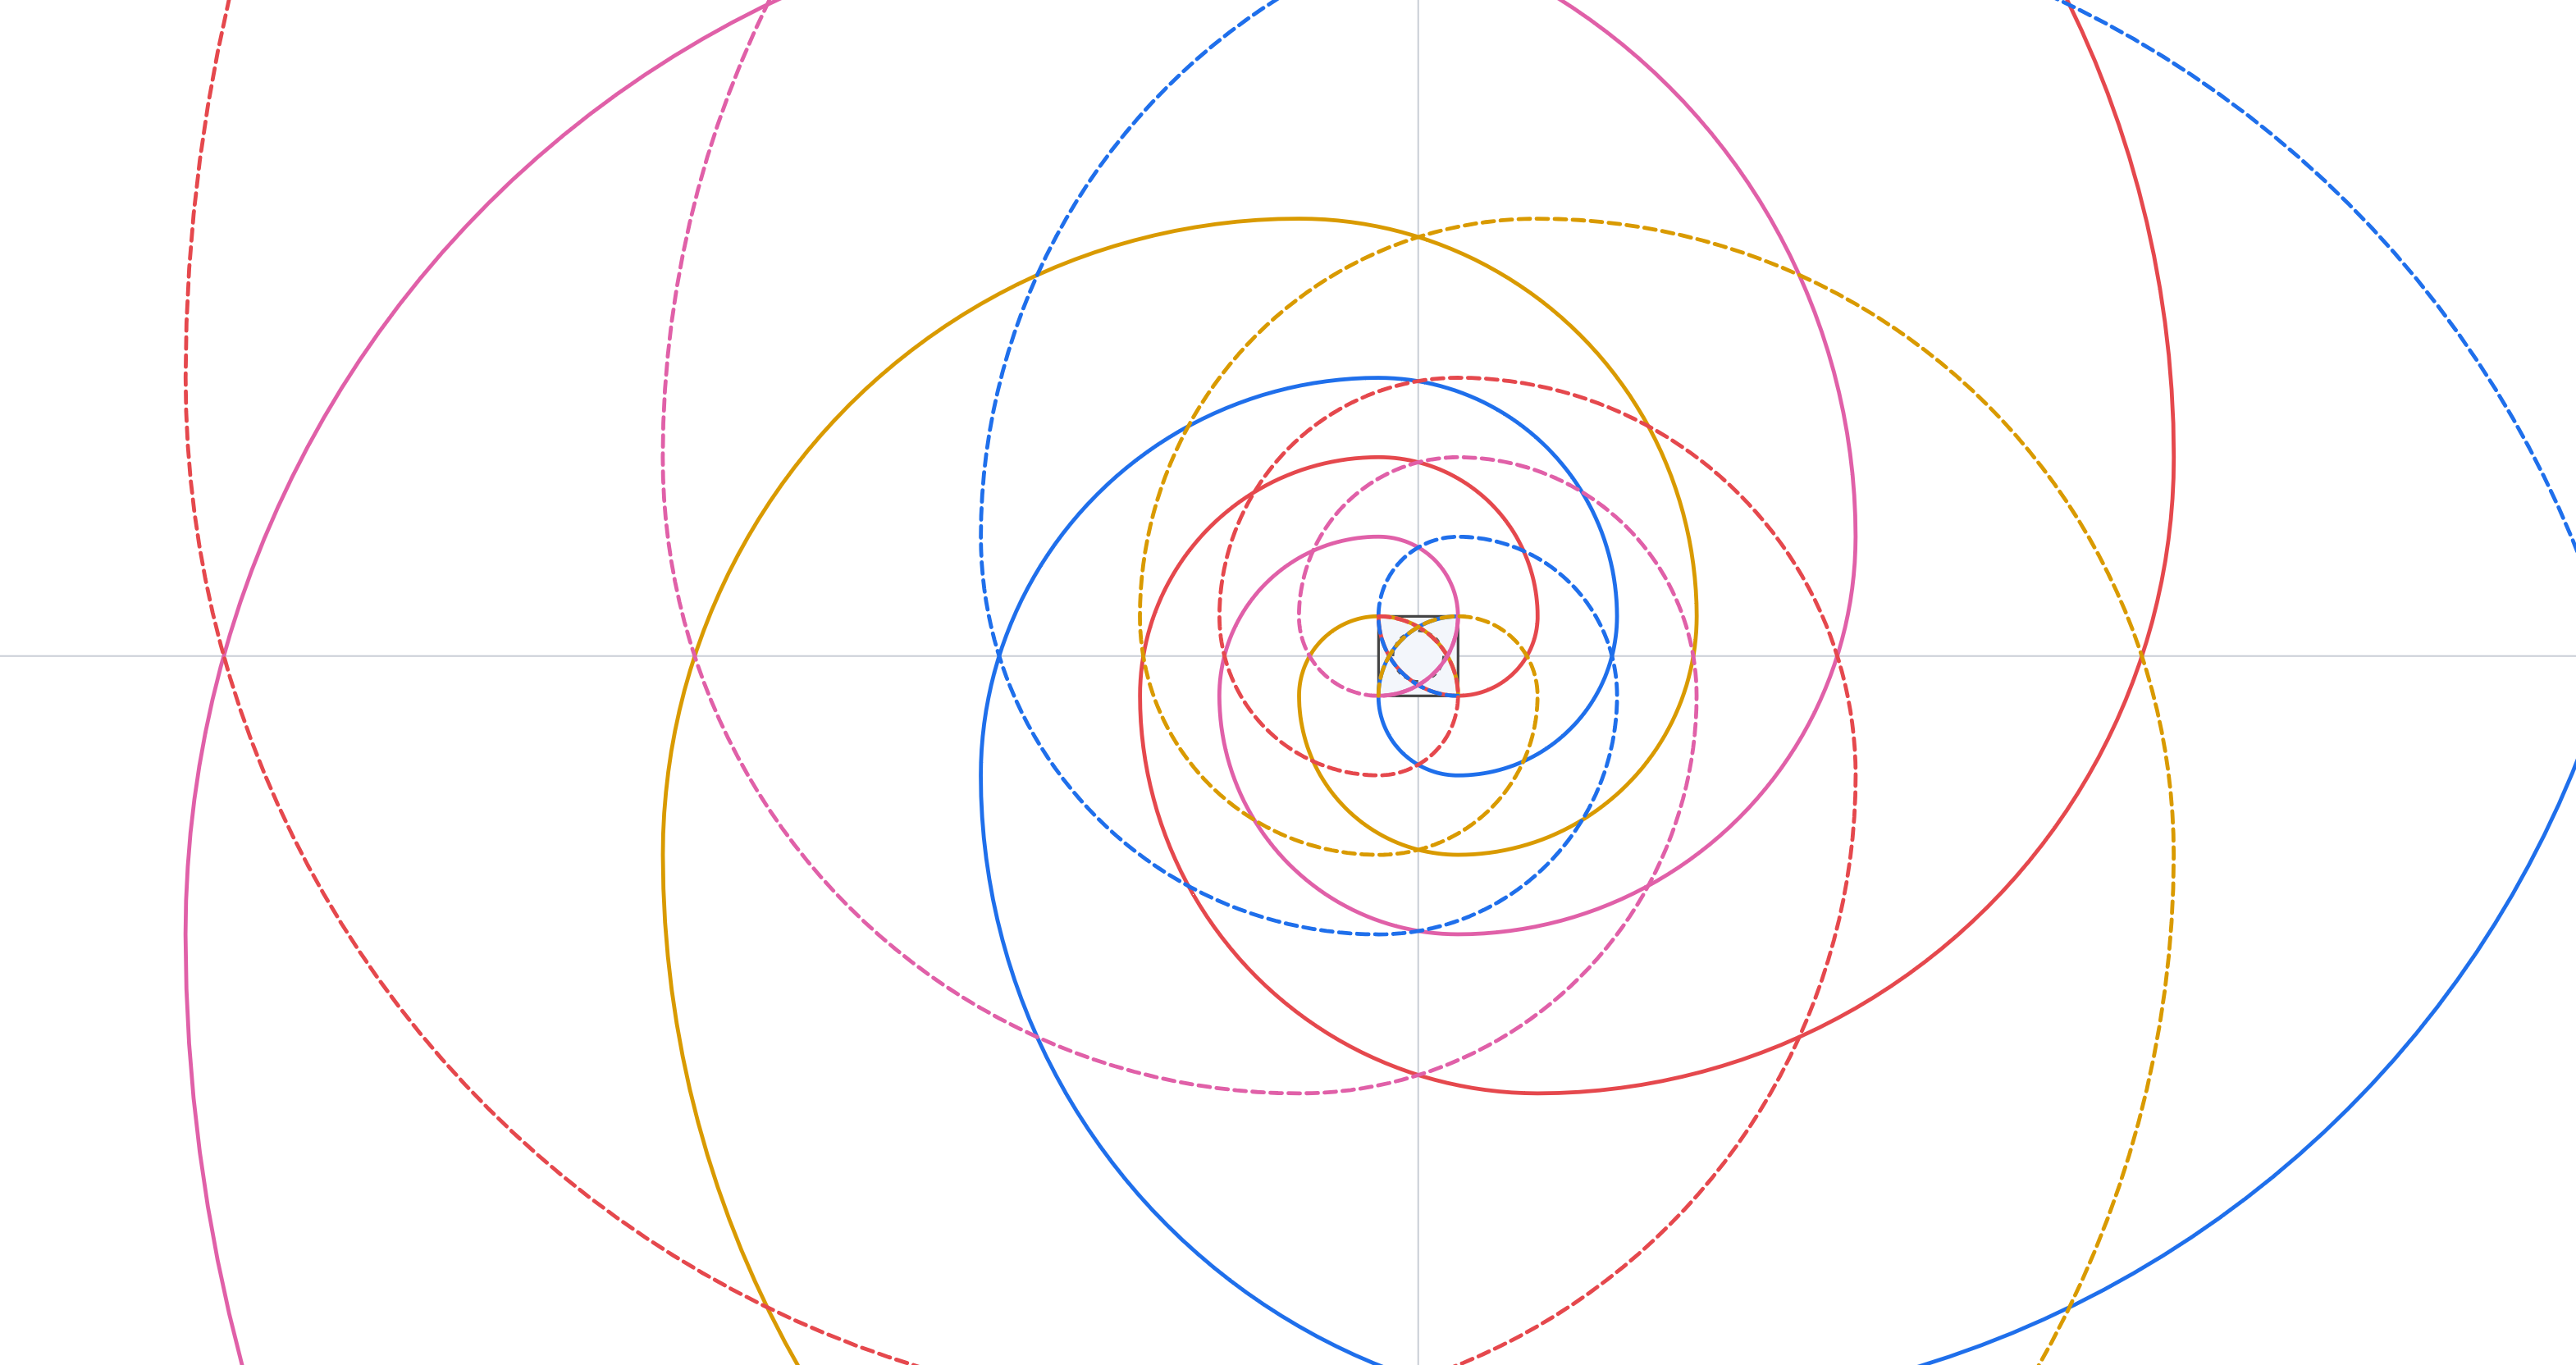
\includegraphics[width=0.5\textwidth]{fig4_spirals.png}
\caption{The eight Fibonacci spirals of Theorem~\ref{thm:eight}, all growing out of the unit square (rotations solid, reflections dashed). Drawn with the author's Spiral Workbench, \url{https://lluisgarcia.github.io/The-Pentametric-Cycle/spiral-workbench/}.}
\label{fig:spirals}
\end{figure}

\section{Connection with Holden's lines}

\begin{proposition}\label{prop:holden}
Holden's two lines are built from the circle of origins at the origin $H_0=(\tfrac3{10},-\tfrac1{10})$, Holden's crossing, where the circle crosses the diagonal arc about $(-\tfrac12,\tfrac12)$:
\begin{enumerate}[label=(\alph*),itemsep=1pt]
\item the \emph{even line} $3x-y=1$, through the centres $C_2,C_4,\dots$ of the even-numbered squares, is the tangent of the circle of origins at $H_0$; it passes through the end $E$ of that arc (Theorem~\ref{thm:unique});
\item the \emph{odd line} $x+3y=0$, through the centres $C_1,C_3,\dots$ of the odd-numbered squares, is the perpendicular to that tangent at $H_0$, extended through $O$ to the opposite origin $Q=-H_0=(-\tfrac3{10},\tfrac1{10})$ on the opposite diagonal arc. It is also a tangent of a circle of the same area $\pi/10$: the circle about the origin $N=(-\tfrac1{10},-\tfrac3{10})$, a quarter turn from $H_0$ (or about $-N$), which it touches at $O$.
\end{enumerate}
They cross at right angles at $H_0$.

\end{proposition}

\begin{proof}
(a) $|H_0|^2=\tfrac1{10}$, and $3x-y=1$ is the line $x\cdot H_0=|H_0|^2$ scaled by $10$; $3\cdot\tfrac12-\tfrac12=1$. (b) The direction $(3,-1)$ of $O H_0$ is the normal of the tangent, so the perpendicular at $H_0$ is the line through $O$ and $H_0$, that is $x+3y=0$, and it meets the circle again at $-H_0$, which lies on the diagonal arc about $(\tfrac12,-\tfrac12)$ since $|-H_0-(\tfrac12,-\tfrac12)|=|(-\tfrac45,\tfrac35)|=1$. The distance from $N$ to $x+3y=0$ is $|{-\tfrac1{10}}-\tfrac9{10}|/\sqrt{10}=1/\sqrt{10}=\rho$, and the foot of the perpendicular is $N+\tfrac1{10}(1,3)=O$.
\end{proof}

The same holds for the whole \emph{origins grid}, the lines $3x-y=1+m$ and $x+3y=m$ ($m\in\mathbb Z$), a tilted square grid with cells of side $\rho$ (called Holden's grid in \cite{rhombus}; Holden's paper has no grid, so we rename it after the origins unit): consecutive lines are $\rho$ apart, so each line is a tangent of the circles of area $\pi/10$ about the nodes next to it. The spacing of the grid is the radius of the circle of origins, and the distances of the centres from $H_0$ are whole multiples of it, $L_k\rho$ (Section~1). Note that $H_0$ does not lie on the spiral's own first arc, which is the arc about $(\tfrac12,-\tfrac12)$; it lies on the first arc of the opposite spiral, the half-turned one. The point $Q=-H_0=(-\tfrac3{10},\tfrac1{10})$, where the odd line crosses the spiral's own first arc and which was the starting point of \cite{rhombus} (there $Q=-P$), is one of the eight origins.

\begin{theorem}[eight origins, eight spirals]\label{thm:eight}
The eight symmetries of the square (four rotations about $O$ and four reflections) map the tiling to eight tilings, each with its own spiral, and map $H_0$ to the eight origins, one each; we call the image of $H_0$ the origin of that tiling (it is that tiling's Holden crossing, and lies on the first arc of the opposite tiling). At each of the eight origins, Holden's lines of its own tiling come from the circle of origins: one is its tangent there, the other the perpendicular to it, through $O$ to the opposite origin (Figure~\ref{fig:spirals}).
\end{theorem}

\begin{proof}
Each symmetry fixes $O$, preserves the circle of origins, permutes the four diagonal arcs, maps origins to origins, and carries tangents to tangents and square centres to square centres. The point $H_0$ lies on no axis of symmetry of the square, so its eight images are distinct, and they are the eight origins of Corollary~\ref{cor:origins}. Proposition~\ref{prop:holden} then holds at every origin for the tiling it belongs to.
\end{proof}



\begin{remark}[opposite spirals share the odd line]
The half turn about $O$ maps the spiral to its opposite. It maps the odd line $x+3y=0$ onto itself, because the line passes through $O$, so both spirals have their odd centres on the same line, which joins their two origins $H_0$ and $-H_0$. Their even lines are different: $3x-y=1$ and $3x-y=-1$, the two parallel tangents of the circle of origins at $H_0$ and at $-H_0$. The same holds for each of the four pairs of opposite origins. Each of Holden's lines has slope $\pm3$ or $\pm\tfrac13$, so it cuts every square whose centre it carries at the thirds of two opposite sides. Thus the odd line cuts the unit square at $(\pm\tfrac12,\mp\tfrac16)$, and the opposite spiral's even line $3x-y=-1$ cuts that spiral's second square, centred at $(0,1)$, at $(-\tfrac16,\tfrac12)$ and $(\tfrac16,\tfrac32)$: the same pattern, turned a quarter turn. Indeed that second square also has side $1$, so it is itself a unit square, with its own origin of origins at its centre $(0,1)$; seen from there, the line $3x-y=-1$, which passes through $(0,1)$ with slope $3$, is the odd line of the tilings that start from that square turned a quarter turn. The line through the even centres of one spiral is, flipped, a line through the odd centres of a spiral that starts from the next unit square.
\end{remark}

\begin{remark}[what is Holden's and what is new]\label{rem:credit}
Holden (1975) proved that the centres lie on two perpendicular lines of slopes $3$ and $-\tfrac13$, and gave their distances from the crossing in closed form; his tables list $d\sqrt{10}$, which for the Fibonacci tiling are the Lucas numbers $3,4,7,11,\dots$ (he does not name them). Gardiner (1984) gave the lines in coordinates centred on the first square, which puts the crossing $1/\sqrt{10}$ from that centre. We have not found the following in \cite{holden} or \cite{gardiner}: that the crossing lies on a diagonal arc of the first square; that the tangent there passes through an end of that arc; that the circle of area $\pi/10$ is the only circle about the centre with this property; and the eight origins and eight spirals that follow. Neither paper uses a grid. In \cite{rhombus} this length was called the Holden unit; here we call it the origins unit.
\end{remark}

The origin of origins is itself a node of the origins grid, so the circle of origins touches the four grid lines next to $O$: at $H_0$, at $Q=-H_0$, and at $\pm(\tfrac1{10},\tfrac3{10})$, four of the eight origins. The other four are the touching points of the mirror-image grid.

\section{Angles, areas and squares}

\begin{proposition}\label{prop:angles}
Seen from $O$, consecutive origins are alternately $\arctan(4/3)=53.13^\circ$ and $\arctan(3/4)=36.87^\circ$ apart, the two acute angles of the $3$-$4$-$5$ triangle. The triangles they form with $O$ have areas exactly $\tfrac4{100}$ and $\tfrac3{100}$, and two consecutive gaps together ($90^\circ$) enclose $\tfrac5{100}$. The chords between consecutive origins are $\sqrt{0.08}$ and $\tfrac15$, in the ratio $\sqrt2$.
\end{proposition}

\begin{proof}
For example $(\tfrac3{10},-\tfrac1{10})$ and $(\tfrac3{10},\tfrac1{10})$ make an angle with $\cos\theta = \tfrac{8/100}{1/10}=\tfrac45$, and $(\tfrac3{10},\tfrac1{10})$, $(\tfrac1{10},\tfrac3{10})$ one with $\cos\theta=\tfrac35$. The area of the triangle is $\tfrac12\rho^2\sin\theta=\tfrac1{20}\sin\theta$, with $\sin\theta = \tfrac35,\tfrac45,1$.
\end{proof}

\begin{proposition}\label{prop:squares}
\begin{enumerate}[label=(\alph*),itemsep=1pt]
\item Alternate origins form two squares, $(\tfrac3{10},\tfrac1{10})$, $(-\tfrac1{10},\tfrac3{10})$, $(-\tfrac3{10},-\tfrac1{10})$, $(\tfrac1{10},-\tfrac3{10})$ and its mirror image, each of side $\sqrt{0.2}$ and area $\tfrac15$: the square on the diagonal of a cell of the origins grid.
\item The tangents to the diagonal arcs at the four vertices of each of these squares are $\tfrac3{10}$ from $O$ and form a square of side $\tfrac35$, area $\tfrac9{25}$.
\item The two squares of (a) cross in eight points at exact $45^\circ$ steps around $O$, at distances $\tfrac14$ and $\tfrac{\sqrt2}{6}$ alternately (Figure~\ref{fig:squares}). These eight points are the vertices of a square of area $\tfrac18$, with vertices $(\pm\tfrac14,0)$, $(0,\pm\tfrac14)$, and a square of area $\tfrac19$ (side $\tfrac13$), with vertices $(\pm\tfrac16,\pm\tfrac16)$.
\end{enumerate}
\end{proposition}

\begin{proof}
(a) The squared distance between alternate origins is $(\tfrac4{10})^2+(\tfrac2{10})^2=\tfrac15$. (b) At $p=(\tfrac3{10},-\tfrac1{10})$ the radius of the arc is $p-(-\tfrac12,\tfrac12)=(\tfrac45,-\tfrac35)$, and $|(\tfrac45,-\tfrac35)\cdot p|=\tfrac3{10}$; the four radii point in two perpendicular directions. (c) The first square is $|x+2y|\le\tfrac12$, $|2x-y|\le\tfrac12$, and its mirror image is $|x-2y|\le\tfrac12$, $|2x+y|\le\tfrac12$. The sides $x+2y=\tfrac12$ and $2x+y=\tfrac12$ meet at $(\tfrac16,\tfrac16)$, and the sides $2x-y=\tfrac12$ and $2x+y=\tfrac12$ at $(\tfrac14,0)$, both inside the segments. The rest follows by the symmetries of the square.
\end{proof}

\begin{figure}[!ht]
\centering
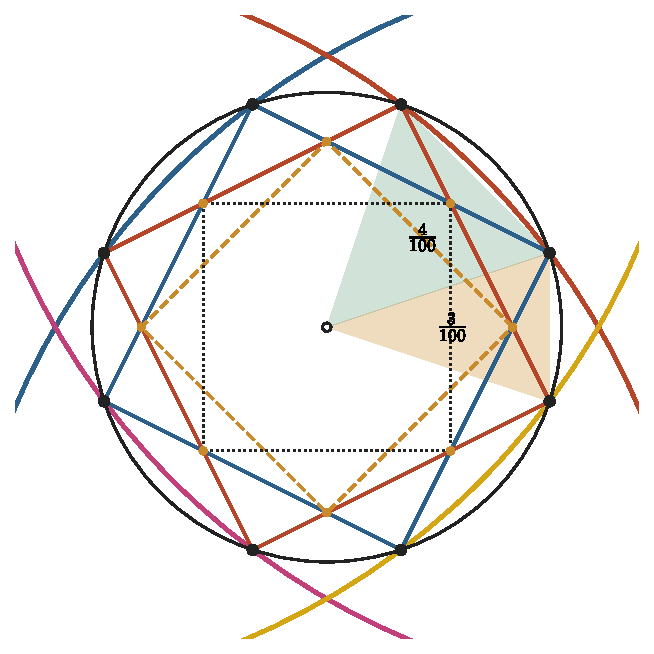
\includegraphics[width=0.3\textwidth]{fig3_squares.pdf}
\caption{The two squares of alternate origins (blue, red; area $1/5$ each) cross in eight points, the vertices of a square of area $1/8$ (gold, dashed) and a square of area $1/9$ (dotted). Shaded: the triangles of areas $3/100$ and $4/100$ between consecutive origins.}
\label{fig:squares}
\end{figure}

\section{Remarks}

\begin{enumerate}[leftmargin=*,itemsep=0pt,topsep=2pt]
\item The construction was first seen from one point, $Q$, which the author called a ``second origin'' (it is the crossing $Q=-P$ of \cite{rhombus}). Theorem~\ref{thm:eight} shows there is nothing second about it: there is one origin of origins, $O$, and eight equal origins around it.
\item Every arc of each of the eight spirals is exactly the diagonal arc of its own square, so each spiral is built, at every size, from one and the same exact shape. The factor from one square to the next, $F_{k+1}/F_k = 1, 2, \tfrac32, \tfrac53, \dots$, is not constant (it tends to the golden ratio), so no single enlargement maps a spiral onto itself; in that sense it differs from the golden spiral. The circle of origins, the eight origins and Holden's lines are exact at every size.
\item The origins unit is also the step of the author's Pentametric spiral \cite{gt}, where the square of area $\mathfrak{P}(n)$ lies $n$ units from the crossing and the perfect squares occur exactly at the Lucas numbers, the Fibonacci squares. That connection will be treated in a separate note.
\item Exact checks: \texttt{verify\_origins.py} (the rational statements exactly, the angles numerically); figures: \texttt{figs\_origins.py}. Repository:\\ \url{https://github.com/lluisgarcia/The-Pentametric-Cycle}.
\end{enumerate}

\paragraph{Acknowledgements and use of AI.} The eight origins, the circle of area $\pi/10$, the reading of Holden's lines as tangents of circles of that size, the observation that circles of other radii give tangents that miss the corner, the eight spirals and the names are the author's, found in GeoGebra and in the Spiral Workbench (an interactive page built for this study with Claude Code). Claude (Anthropic, Opus 5.5) was used to verify the statements in exact arithmetic, to put the uniqueness in algebraic form, to prepare the figures and to help draft the text; the author checked and approved every statement. Licence: CC BY 4.0 for this note, MIT for the Python scripts.

{\footnotesize\begin{thebibliography}{9}\setlength{\itemsep}{0pt}
\bibitem{holden} H.~L. Holden, Fibonacci tiles, \emph{The Fibonacci Quarterly} \textbf{13} (1975) 45--49.
\bibitem{gardiner} T. Gardiner, 68.15 The Fibonacci spiral, \emph{The Mathematical Gazette} \textbf{68} (1984) 120.
\bibitem{rhombus} L. Garcia Torcal, \emph{The Epitetartic Rhombus}, note, Zenodo (2026), \href{https://doi.org/10.5281/zenodo.23325442}{doi:10.5281/zenodo.23325442}.
\bibitem{gt} L. Garcia Torcal, \emph{The Pentametric Cycle: A Nested Palindrome Encoding the Pythagorean Consonances}, preprint, Zenodo (2026), \href{https://doi.org/10.5281/zenodo.23183108}{doi:10.5281/zenodo.23183108}.
\end{thebibliography}}

\end{document}
